\documentclass{standalone}
\usepackage{tikz}
\usetikzlibrary{patterns, positioning}

\begin{document}
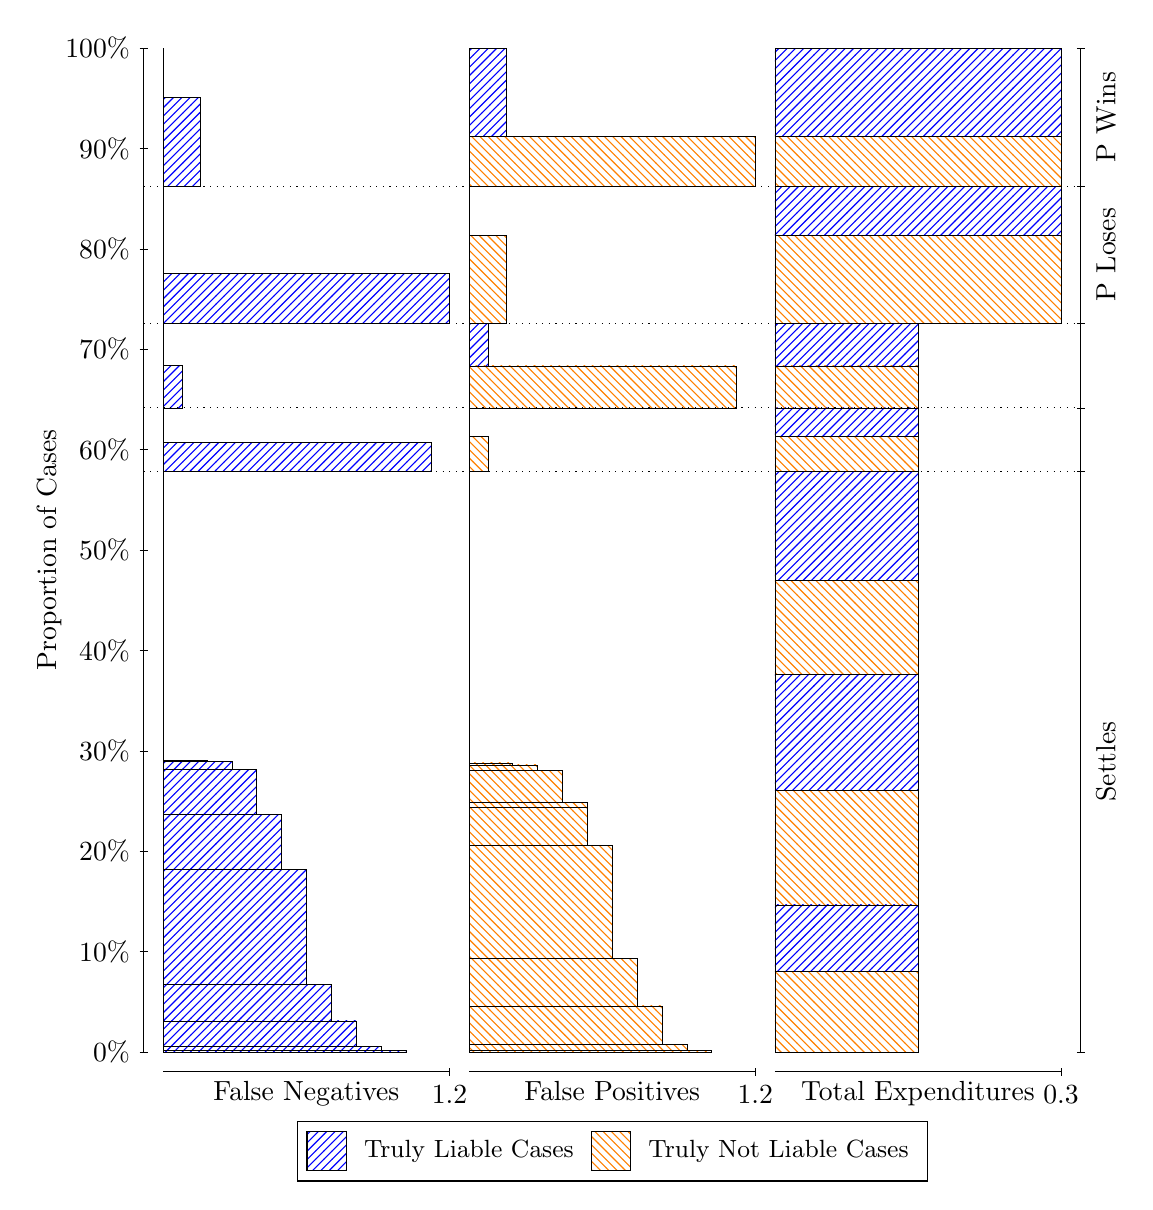
\begin{tikzpicture}
\draw[black, very thin] (1.5,1.75) -- (1.5,14.5);
\node[rotate=90, anchor=center] at (0.3, 8.125) {Proportion of Cases};
\draw[black, very thin] (1.45,1.75) -- (1.55,1.75);
\node[anchor=east] at (1.45, 1.75) {0\%};
\draw[black, very thin] (1.45,3.025) -- (1.55,3.025);
\node[anchor=east] at (1.45, 3.025) {10\%};
\draw[black, very thin] (1.45,4.3) -- (1.55,4.3);
\node[anchor=east] at (1.45, 4.3) {20\%};
\draw[black, very thin] (1.45,5.575) -- (1.55,5.575);
\node[anchor=east] at (1.45, 5.575) {30\%};
\draw[black, very thin] (1.45,6.85) -- (1.55,6.85);
\node[anchor=east] at (1.45, 6.85) {40\%};
\draw[black, very thin] (1.45,8.125) -- (1.55,8.125);
\node[anchor=east] at (1.45, 8.125) {50\%};
\draw[black, very thin] (1.45,9.4) -- (1.55,9.4);
\node[anchor=east] at (1.45, 9.4) {60\%};
\draw[black, very thin] (1.45,10.675) -- (1.55,10.675);
\node[anchor=east] at (1.45, 10.675) {70\%};
\draw[black, very thin] (1.45,11.95) -- (1.55,11.95);
\node[anchor=east] at (1.45, 11.95) {80\%};
\draw[black, very thin] (1.45,13.225) -- (1.55,13.225);
\node[anchor=east] at (1.45, 13.225) {90\%};
\draw[black, very thin] (1.45,14.5) -- (1.55,14.5);
\node[anchor=east] at (1.45, 14.5) {100\%};

\draw[black, very thin] (13.4,1.75) -- (13.4,14.5);
\draw[black, very thin] (13.35,1.75) -- (13.45,1.75);
\node[anchor=west] at (13.35, 1.75) {};
\draw[black, very thin] (13.35,9.1276) -- (13.45,9.1276);
\node[anchor=west] at (13.35, 9.1276) {};
\draw[black, very thin] (13.35,9.9312) -- (13.45,9.9312);
\node[anchor=west] at (13.35, 9.9312) {};
\draw[black, very thin] (13.35,11.007) -- (13.45,11.007);
\node[anchor=west] at (13.35, 11.007) {};
\draw[black, very thin] (13.35,12.747) -- (13.45,12.747);
\node[anchor=west] at (13.35, 12.747) {};
\draw[black, very thin] (13.35,14.5) -- (13.45,14.5);
\node[anchor=west] at (13.35, 14.5) {};

\draw[black, very thin, pattern color=blue, pattern=north east lines] (1.75,1.75) rectangle (4.8304,1.7657);
\draw[black, very thin, pattern color=blue, pattern=north east lines] (1.75,1.7657) rectangle (4.5145,1.8219);
\draw[black, very thin, pattern color=blue, pattern=north east lines] (1.75,1.8219) rectangle (4.1986,2.1444);
\draw[black, very thin, pattern color=blue, pattern=north east lines] (1.75,2.1444) rectangle (3.8826,2.6083);
\draw[black, very thin, pattern color=blue, pattern=north east lines] (1.75,2.6083) rectangle (3.5667,4.0717);
\draw[black, very thin, pattern color=blue, pattern=north east lines] (1.75,4.0717) rectangle (3.2507,4.7686);
\draw[black, very thin, pattern color=blue, pattern=north east lines] (1.75,4.7686) rectangle (2.9348,5.3434);
\draw[black, very thin, pattern color=blue, pattern=north east lines] (1.75,5.3434) rectangle (2.6188,5.4372);
\draw[black, very thin, pattern color=blue, pattern=north east lines] (1.75,5.4372) rectangle (2.3029,5.4575);
\draw[black, very thin, pattern color=orange, pattern=north west lines] (1.75,5.4575) rectangle (1.75,9.1276);
\draw[black, very thin, pattern color=blue, pattern=north east lines] (1.75,9.1276) rectangle (5.1464,9.4941);
\draw[black, very thin, pattern color=orange, pattern=north west lines] (1.75,9.4941) rectangle (1.75,9.9312);
\draw[black, very thin, pattern color=blue, pattern=north east lines] (1.75,9.9312) rectangle (1.987,10.474);
\draw[black, very thin, pattern color=orange, pattern=north west lines] (1.75,10.474) rectangle (1.75,11.007);
\draw[black, very thin, pattern color=blue, pattern=north east lines] (1.75,11.007) rectangle (5.3833,11.638);
\draw[black, very thin, pattern color=orange, pattern=north west lines] (1.75,11.638) rectangle (1.75,12.747);
\draw[black, very thin, pattern color=blue, pattern=north east lines] (1.75,12.747) rectangle (2.2239,13.874);
\draw[black, very thin, pattern color=orange, pattern=north west lines] (1.75,13.874) rectangle (1.75,14.5);
\draw[black, very thin, pattern color=orange, pattern=north west lines] (5.6333,1.75) rectangle (8.7138,1.7658);
\draw[black, very thin, pattern color=orange, pattern=north west lines] (5.6333,1.7658) rectangle (8.3978,1.8459);
\draw[black, very thin, pattern color=orange, pattern=north west lines] (5.6333,1.8459) rectangle (8.0819,2.3352);
\draw[black, very thin, pattern color=orange, pattern=north west lines] (5.6333,2.3352) rectangle (7.7659,2.9423);
\draw[black, very thin, pattern color=orange, pattern=north west lines] (5.6333,2.9423) rectangle (7.45,4.3697);
\draw[black, very thin, pattern color=orange, pattern=north west lines] (5.6333,4.3697) rectangle (7.1341,4.8567);
\draw[black, very thin, pattern color=orange, pattern=north west lines] (5.6333,4.8567) rectangle (7.1341,4.9164);
\draw[black, very thin, pattern color=orange, pattern=north west lines] (5.6333,4.9164) rectangle (6.8181,5.323);
\draw[black, very thin, pattern color=orange, pattern=north west lines] (5.6333,5.323) rectangle (6.5022,5.3962);
\draw[black, very thin, pattern color=orange, pattern=north west lines] (5.6333,5.3962) rectangle (6.1862,5.4201);
\draw[black, very thin, pattern color=blue, pattern=north east lines] (5.6333,5.4201) rectangle (5.6333,9.1276);
\draw[black, very thin, pattern color=orange, pattern=north west lines] (5.6333,9.1276) rectangle (5.8703,9.5647);
\draw[black, very thin, pattern color=blue, pattern=north east lines] (5.6333,9.5647) rectangle (5.6333,9.9312);
\draw[black, very thin, pattern color=orange, pattern=north west lines] (5.6333,9.9312) rectangle (9.0297,10.464);
\draw[black, very thin, pattern color=blue, pattern=north east lines] (5.6333,10.464) rectangle (5.8703,11.007);
\draw[black, very thin, pattern color=orange, pattern=north west lines] (5.6333,11.007) rectangle (6.1072,12.116);
\draw[black, very thin, pattern color=blue, pattern=north east lines] (5.6333,12.116) rectangle (5.6333,12.747);
\draw[black, very thin, pattern color=orange, pattern=north west lines] (5.6333,12.747) rectangle (9.2667,13.374);
\draw[black, very thin, pattern color=blue, pattern=north east lines] (5.6333,13.374) rectangle (6.1072,14.5);
\draw[black, very thin, pattern color=orange, pattern=north west lines] (9.5167,1.75) rectangle (11.333,2.7765);
\draw[black, very thin, pattern color=blue, pattern=north east lines] (9.5167,2.7765) rectangle (11.333,3.6191);
\draw[black, very thin, pattern color=orange, pattern=north west lines] (9.5167,3.6191) rectangle (11.333,5.0704);
\draw[black, very thin, pattern color=blue, pattern=north east lines] (9.5167,5.0704) rectangle (11.333,6.5495);
\draw[black, very thin, pattern color=orange, pattern=north west lines] (9.5167,6.5495) rectangle (11.333,7.7418);
\draw[black, very thin, pattern color=blue, pattern=north east lines] (9.5167,7.7418) rectangle (11.333,9.1276);
\draw[black, very thin, pattern color=orange, pattern=north west lines] (9.5167,9.1276) rectangle (11.333,9.5647);
\draw[black, very thin, pattern color=blue, pattern=north east lines] (9.5167,9.5647) rectangle (11.333,9.9312);
\draw[black, very thin, pattern color=orange, pattern=north west lines] (9.5167,9.9312) rectangle (11.333,10.464);
\draw[black, very thin, pattern color=blue, pattern=north east lines] (9.5167,10.464) rectangle (11.333,11.007);
\draw[black, very thin, pattern color=orange, pattern=north west lines] (9.5167,11.007) rectangle (13.15,12.116);
\draw[black, very thin, pattern color=blue, pattern=north east lines] (9.5167,12.116) rectangle (13.15,12.747);
\draw[black, very thin, pattern color=orange, pattern=north west lines] (9.5167,12.747) rectangle (13.15,13.374);
\draw[black, very thin, pattern color=blue, pattern=north east lines] (9.5167,13.374) rectangle (13.15,14.5);
\draw[black, dotted] (1.5,9.1276) -- (13.4,9.1276);
\draw[black, dotted] (1.5,9.9312) -- (13.4,9.9312);
\draw[black, dotted] (1.5,11.007) -- (13.4,11.007);
\draw[black, dotted] (1.5,12.747) -- (13.4,12.747);
\draw[black, very thin] (1.75,1.5) -- (5.3833,1.5);
\node[anchor=north] at (3.5667, 1.5) {False Negatives};
\draw[black, very thin] (5.3833,1.45) -- (5.3833,1.55);
\node[anchor=north] at (5.3833, 1.45) {1.2};

\draw[black, very thin] (5.6333,1.5) -- (9.2667,1.5);
\node[anchor=north] at (7.45, 1.5) {False Positives};
\draw[black, very thin] (9.2667,1.45) -- (9.2667,1.55);
\node[anchor=north] at (9.2667, 1.45) {1.2};

\draw[black, very thin] (9.5167,1.5) -- (13.15,1.5);
\node[anchor=north] at (11.333, 1.5) {Total Expenditures};
\draw[black, very thin] (13.15,1.45) -- (13.15,1.55);
\node[anchor=north] at (13.15, 1.45) {0.3};

\node[black, centered, rotate=90] at (13.72, 5.4388) {Settles};


\node[black, centered, rotate=90] at (13.72, 11.877) {P Loses};
\node[black, centered, rotate=90] at (13.72, 13.624) {P Wins};

\draw (7.449999999999999,1.5) node[draw=none] (baseCoordinate) {};
\begin{scope}[align=center]
        \matrix[scale=0.5, draw=black, below=0.5cm of baseCoordinate, nodes={draw}, column sep=0.1cm]{
            \node[rectangle, draw, minimum width=0.5cm, minimum height=0.5cm, pattern=north east lines, pattern color=blue] {}; &
            \node[draw=none, font=\small] (B) {Truly Liable Cases}; &
            \node[rectangle, draw, minimum width=0.5cm, minimum height=0.5cm, pattern=north west lines, pattern color=orange] {}; &
            \node[draw=none, font=\small] (B) {Truly Not Liable Cases}; \\
            };
\end{scope}

\end{tikzpicture}
\end{document}